We will now describe and discuss the results of our simulations. For the whole study we used a number  $N=1000$ of helium atoms. It is a compromise between realistic size to compare with experiments (typical droplet sizes between $\sim$ 500 and $\sim$ 10000 atoms for this type of measurements) and computational cost.

\section{Finding ground state properties}

($4s$) state is the ground state of our system. 
Thanks to the moderate computational cost of its simulation we can examine several important factors.
The first one is the comparison of a classical \textit{vs} quantum treatment of the potassium atom.
The second one is the version of the functional used, the original OT one or a modification designed to deal with high values of the density described as solid functional in \citsec{sec:DFT-func-analytics}.

\subsection{Quantum versus classical potassium}
\label{sec:4S-dia}

The ground state K wave function is expected to be smooth.
Hence it can be described using the same grid as the helium one. 
As can be seen in \citfig{fig:4S-Q-C-lsolid}, a quantum treatment of the potassium atom leads to a slightly displaced atom from center of mass of the droplet (around 1\AA) compared to the position given by a classical description.
In addition, the droplet radius is slightly increased and the surface region slightly more diffuse.
This phenomenon can be understood by considering the spatial extension of the impurity wave-function compared to the classical point-like position.
\begin{figure}[h]
	\centering
	% GNUPLOT: LaTeX picture with Postscript
\begingroup
  \makeatletter
  \providecommand\color[2][]{%
    \GenericError{(gnuplot) \space\space\space\@spaces}{%
      Package color not loaded in conjunction with
      terminal option `colourtext'%
    }{See the gnuplot documentation for explanation.%
    }{Either use 'blacktext' in gnuplot or load the package
      color.sty in LaTeX.}%
    \renewcommand\color[2][]{}%
  }%
  \providecommand\includegraphics[2][]{%
    \GenericError{(gnuplot) \space\space\space\@spaces}{%
      Package graphicx or graphics not loaded%
    }{See the gnuplot documentation for explanation.%
    }{The gnuplot epslatex terminal needs graphicx.sty or graphics.sty.}%
    \renewcommand\includegraphics[2][]{}%
  }%
  \providecommand\rotatebox[2]{#2}%
  \@ifundefined{ifGPcolor}{%
    \newif\ifGPcolor
    \GPcolortrue
  }{}%
  \@ifundefined{ifGPblacktext}{%
    \newif\ifGPblacktext
    \GPblacktextfalse
  }{}%
  % define a \g@addto@macro without @ in the name:
  \let\gplgaddtomacro\g@addto@macro
  % define empty templates for all commands taking text:
  \gdef\gplbacktext{}%
  \gdef\gplfronttext{}%
  \makeatother
  \ifGPblacktext
    % no textcolor at all
    \def\colorrgb#1{}%
    \def\colorgray#1{}%
  \else
    % gray or color?
    \ifGPcolor
      \def\colorrgb#1{\color[rgb]{#1}}%
      \def\colorgray#1{\color[gray]{#1}}%
      \expandafter\def\csname LTw\endcsname{\color{white}}%
      \expandafter\def\csname LTb\endcsname{\color{black}}%
      \expandafter\def\csname LTa\endcsname{\color{black}}%
      \expandafter\def\csname LT0\endcsname{\color[rgb]{1,0,0}}%
      \expandafter\def\csname LT1\endcsname{\color[rgb]{0,1,0}}%
      \expandafter\def\csname LT2\endcsname{\color[rgb]{0,0,1}}%
      \expandafter\def\csname LT3\endcsname{\color[rgb]{1,0,1}}%
      \expandafter\def\csname LT4\endcsname{\color[rgb]{0,1,1}}%
      \expandafter\def\csname LT5\endcsname{\color[rgb]{1,1,0}}%
      \expandafter\def\csname LT6\endcsname{\color[rgb]{0,0,0}}%
      \expandafter\def\csname LT7\endcsname{\color[rgb]{1,0.3,0}}%
      \expandafter\def\csname LT8\endcsname{\color[rgb]{0.5,0.5,0.5}}%
    \else
      % gray
      \def\colorrgb#1{\color{black}}%
      \def\colorgray#1{\color[gray]{#1}}%
      \expandafter\def\csname LTw\endcsname{\color{white}}%
      \expandafter\def\csname LTb\endcsname{\color{black}}%
      \expandafter\def\csname LTa\endcsname{\color{black}}%
      \expandafter\def\csname LT0\endcsname{\color{black}}%
      \expandafter\def\csname LT1\endcsname{\color{black}}%
      \expandafter\def\csname LT2\endcsname{\color{black}}%
      \expandafter\def\csname LT3\endcsname{\color{black}}%
      \expandafter\def\csname LT4\endcsname{\color{black}}%
      \expandafter\def\csname LT5\endcsname{\color{black}}%
      \expandafter\def\csname LT6\endcsname{\color{black}}%
      \expandafter\def\csname LT7\endcsname{\color{black}}%
      \expandafter\def\csname LT8\endcsname{\color{black}}%
    \fi
  \fi
    \setlength{\unitlength}{0.0500bp}%
    \ifx\gptboxheight\undefined%
      \newlength{\gptboxheight}%
      \newlength{\gptboxwidth}%
      \newsavebox{\gptboxtext}%
    \fi%
    \setlength{\fboxrule}{0.5pt}%
    \setlength{\fboxsep}{1pt}%
\begin{picture}(10080.00,2880.00)%
    \gplgaddtomacro\gplbacktext{%
      \csname LTb\endcsname%
      \put(1078,704){\makebox(0,0)[r]{\strut{}$0$}}%
      \csname LTb\endcsname%
      \put(1078,1086){\makebox(0,0)[r]{\strut{}$0.005$}}%
      \csname LTb\endcsname%
      \put(1078,1468){\makebox(0,0)[r]{\strut{}$0.01$}}%
      \csname LTb\endcsname%
      \put(1078,1851){\makebox(0,0)[r]{\strut{}$0.015$}}%
      \csname LTb\endcsname%
      \put(1078,2233){\makebox(0,0)[r]{\strut{}$0.02$}}%
      \csname LTb\endcsname%
      \put(1078,2615){\makebox(0,0)[r]{\strut{}$0.025$}}%
      \csname LTb\endcsname%
      \put(1210,484){\makebox(0,0){\strut{}$0$}}%
      \csname LTb\endcsname%
      \put(1832,484){\makebox(0,0){\strut{}$5$}}%
      \csname LTb\endcsname%
      \put(2454,484){\makebox(0,0){\strut{}$10$}}%
      \csname LTb\endcsname%
      \put(3075,484){\makebox(0,0){\strut{}$15$}}%
      \csname LTb\endcsname%
      \put(3697,484){\makebox(0,0){\strut{}$20$}}%
      \csname LTb\endcsname%
      \put(4319,484){\makebox(0,0){\strut{}$25$}}%
      \csname LTb\endcsname%
      \put(4941,484){\makebox(0,0){\strut{}$30$}}%
      \csname LTb\endcsname%
      \put(5562,484){\makebox(0,0){\strut{}$35$}}%
      \csname LTb\endcsname%
      \put(6184,484){\makebox(0,0){\strut{}$40$}}%
      \csname LTb\endcsname%
      \put(6806,484){\makebox(0,0){\strut{}$45$}}%
      \csname LTb\endcsname%
      \put(7428,484){\makebox(0,0){\strut{}$50$}}%
      \csname LTb\endcsname%
      \put(8049,484){\makebox(0,0){\strut{}$55$}}%
      \csname LTb\endcsname%
      \put(8671,484){\makebox(0,0){\strut{}$60$}}%
      \put(8803,704){\makebox(0,0)[l]{\strut{}$0$}}%
      \put(8803,1086){\makebox(0,0)[l]{\strut{}$0.25$}}%
      \put(8803,1468){\makebox(0,0)[l]{\strut{}$0.5$}}%
      \put(8803,1851){\makebox(0,0)[l]{\strut{}$0.75$}}%
      \put(8803,2233){\makebox(0,0)[l]{\strut{}$1$}}%
      \put(8803,2615){\makebox(0,0)[l]{\strut{}$1.25$}}%
    }%
    \gplgaddtomacro\gplfronttext{%
      \csname LTb\endcsname%
      \put(176,1659){\rotatebox{-270}{\makebox(0,0){\strut{}Helium density (\AA$^{-3}$)}}}%
      \put(9572,1659){\rotatebox{-270}{\makebox(0,0){\strut{}K wave function (\AA$^{-3/2}$)}}}%
      \put(4940,154){\makebox(0,0){\strut{}Position (\AA)}}%
      \csname LTb\endcsname%
      \put(5107,1769){\makebox(0,0)[r]{\strut{}Classical}}%
      \csname LTb\endcsname%
      \put(5107,1549){\makebox(0,0)[r]{\strut{}Quantum}}%
    }%
    \gplbacktext
    \put(0,0){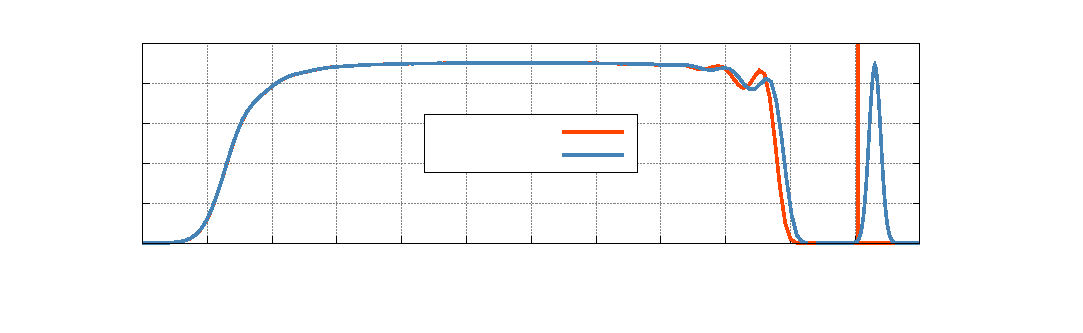
\includegraphics{4S-Q-C-lsolid}}%
    \gplfronttext
  \end{picture}%
\endgroup

	\vspace{-0.5\baselineskip}
	\caption{Density profile in a plane containing the center of mass of the droplet and the potassium atom, for a quantum or a classical description of K}
	\label{fig:4S-Q-C-lsolid}
\end{figure}

\subsection{Quick discussion on the influence of the version of the functional}

We already discussed the fact that the OTC functional could become unstable during a dynamics simulation due to the fact that it cannot handle sharp features appearing around attractive dopants. 
This can occur in the excited ($4p$) states because of the attractive $\Pi$ well. 
The two versions can be compared in the static study of the ground ($4s$) state.
We see in \citfig{fig:4S-C-otc-lsolid} that the two functionals give nearly the same helium density, except near the dopant where the solid version gives a smoother profile, as expected.
\begin{figure}[h]
	\centering
	% GNUPLOT: LaTeX picture with Postscript
\begingroup
  \makeatletter
  \providecommand\color[2][]{%
    \GenericError{(gnuplot) \space\space\space\@spaces}{%
      Package color not loaded in conjunction with
      terminal option `colourtext'%
    }{See the gnuplot documentation for explanation.%
    }{Either use 'blacktext' in gnuplot or load the package
      color.sty in LaTeX.}%
    \renewcommand\color[2][]{}%
  }%
  \providecommand\includegraphics[2][]{%
    \GenericError{(gnuplot) \space\space\space\@spaces}{%
      Package graphicx or graphics not loaded%
    }{See the gnuplot documentation for explanation.%
    }{The gnuplot epslatex terminal needs graphicx.sty or graphics.sty.}%
    \renewcommand\includegraphics[2][]{}%
  }%
  \providecommand\rotatebox[2]{#2}%
  \@ifundefined{ifGPcolor}{%
    \newif\ifGPcolor
    \GPcolortrue
  }{}%
  \@ifundefined{ifGPblacktext}{%
    \newif\ifGPblacktext
    \GPblacktextfalse
  }{}%
  % define a \g@addto@macro without @ in the name:
  \let\gplgaddtomacro\g@addto@macro
  % define empty templates for all commands taking text:
  \gdef\gplbacktext{}%
  \gdef\gplfronttext{}%
  \makeatother
  \ifGPblacktext
    % no textcolor at all
    \def\colorrgb#1{}%
    \def\colorgray#1{}%
  \else
    % gray or color?
    \ifGPcolor
      \def\colorrgb#1{\color[rgb]{#1}}%
      \def\colorgray#1{\color[gray]{#1}}%
      \expandafter\def\csname LTw\endcsname{\color{white}}%
      \expandafter\def\csname LTb\endcsname{\color{black}}%
      \expandafter\def\csname LTa\endcsname{\color{black}}%
      \expandafter\def\csname LT0\endcsname{\color[rgb]{1,0,0}}%
      \expandafter\def\csname LT1\endcsname{\color[rgb]{0,1,0}}%
      \expandafter\def\csname LT2\endcsname{\color[rgb]{0,0,1}}%
      \expandafter\def\csname LT3\endcsname{\color[rgb]{1,0,1}}%
      \expandafter\def\csname LT4\endcsname{\color[rgb]{0,1,1}}%
      \expandafter\def\csname LT5\endcsname{\color[rgb]{1,1,0}}%
      \expandafter\def\csname LT6\endcsname{\color[rgb]{0,0,0}}%
      \expandafter\def\csname LT7\endcsname{\color[rgb]{1,0.3,0}}%
      \expandafter\def\csname LT8\endcsname{\color[rgb]{0.5,0.5,0.5}}%
    \else
      % gray
      \def\colorrgb#1{\color{black}}%
      \def\colorgray#1{\color[gray]{#1}}%
      \expandafter\def\csname LTw\endcsname{\color{white}}%
      \expandafter\def\csname LTb\endcsname{\color{black}}%
      \expandafter\def\csname LTa\endcsname{\color{black}}%
      \expandafter\def\csname LT0\endcsname{\color{black}}%
      \expandafter\def\csname LT1\endcsname{\color{black}}%
      \expandafter\def\csname LT2\endcsname{\color{black}}%
      \expandafter\def\csname LT3\endcsname{\color{black}}%
      \expandafter\def\csname LT4\endcsname{\color{black}}%
      \expandafter\def\csname LT5\endcsname{\color{black}}%
      \expandafter\def\csname LT6\endcsname{\color{black}}%
      \expandafter\def\csname LT7\endcsname{\color{black}}%
      \expandafter\def\csname LT8\endcsname{\color{black}}%
    \fi
  \fi
    \setlength{\unitlength}{0.0500bp}%
    \ifx\gptboxheight\undefined%
      \newlength{\gptboxheight}%
      \newlength{\gptboxwidth}%
      \newsavebox{\gptboxtext}%
    \fi%
    \setlength{\fboxrule}{0.5pt}%
    \setlength{\fboxsep}{1pt}%
\begin{picture}(10080.00,2880.00)%
    \gplgaddtomacro\gplbacktext{%
      \csname LTb\endcsname%
      \put(1078,704){\makebox(0,0)[r]{\strut{}$0$}}%
      \csname LTb\endcsname%
      \put(1078,1086){\makebox(0,0)[r]{\strut{}$0.005$}}%
      \csname LTb\endcsname%
      \put(1078,1468){\makebox(0,0)[r]{\strut{}$0.01$}}%
      \csname LTb\endcsname%
      \put(1078,1851){\makebox(0,0)[r]{\strut{}$0.015$}}%
      \csname LTb\endcsname%
      \put(1078,2233){\makebox(0,0)[r]{\strut{}$0.02$}}%
      \csname LTb\endcsname%
      \put(1078,2615){\makebox(0,0)[r]{\strut{}$0.025$}}%
      \csname LTb\endcsname%
      \put(1210,484){\makebox(0,0){\strut{}$0$}}%
      \csname LTb\endcsname%
      \put(1916,484){\makebox(0,0){\strut{}$5$}}%
      \csname LTb\endcsname%
      \put(2622,484){\makebox(0,0){\strut{}$10$}}%
      \csname LTb\endcsname%
      \put(3328,484){\makebox(0,0){\strut{}$15$}}%
      \csname LTb\endcsname%
      \put(4034,484){\makebox(0,0){\strut{}$20$}}%
      \csname LTb\endcsname%
      \put(4740,484){\makebox(0,0){\strut{}$25$}}%
      \csname LTb\endcsname%
      \put(5447,484){\makebox(0,0){\strut{}$30$}}%
      \csname LTb\endcsname%
      \put(6153,484){\makebox(0,0){\strut{}$35$}}%
      \csname LTb\endcsname%
      \put(6859,484){\makebox(0,0){\strut{}$40$}}%
      \csname LTb\endcsname%
      \put(7565,484){\makebox(0,0){\strut{}$45$}}%
      \csname LTb\endcsname%
      \put(8271,484){\makebox(0,0){\strut{}$50$}}%
      \csname LTb\endcsname%
      \put(8977,484){\makebox(0,0){\strut{}$55$}}%
      \csname LTb\endcsname%
      \put(9683,484){\makebox(0,0){\strut{}$60$}}%
    }%
    \gplgaddtomacro\gplfronttext{%
      \csname LTb\endcsname%
      \put(176,1659){\rotatebox{-270}{\makebox(0,0){\strut{}Helium density (\AA$^{-3}$)}}}%
      \put(5446,154){\makebox(0,0){\strut{}Position (\AA)}}%
      \csname LTb\endcsname%
      \put(5349,1769){\makebox(0,0)[r]{\strut{}Solid}}%
      \csname LTb\endcsname%
      \put(5349,1549){\makebox(0,0)[r]{\strut{}OTC}}%
    }%
    \gplbacktext
    \put(0,0){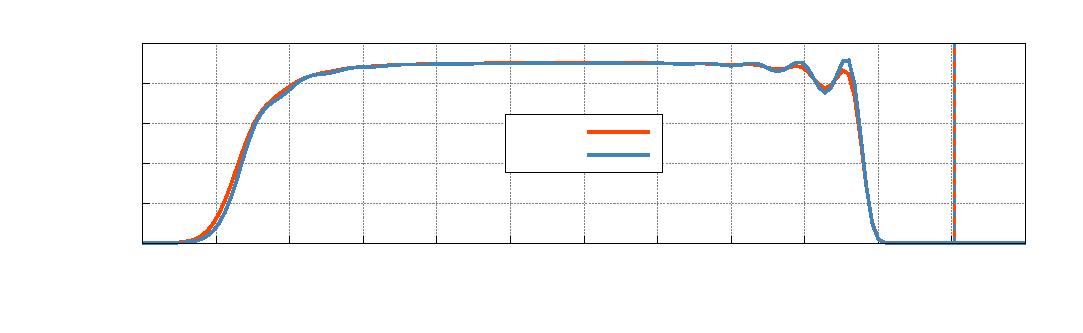
\includegraphics{4S-C-otc-lsolid}}%
    \gplfronttext
  \end{picture}%
\endgroup

	\vspace{-0.5\baselineskip}
	\caption{Density profile in a plane containing the center of mass of the droplet and the potassium atom, for the solid or the OTC functional}
	\label{fig:4S-C-otc-lsolid}
\end{figure}

\subsection{Justifying diabatic hypothesis}

One model that has been very much used to interpret experimental spectra of alkali atoms bound to helium droplets or even some of the dynamics aspects of their photodissociation is the so-called \emph{pseudo-diatomic model}.
In this model the system is represented as a diatomic molecule in which the helium droplet plays the role of a pseudo-atom.
The potential energy curves for this model are then taken by averaging the pair potentials over the (static) helium density. \\

There are two ways of choosing which density to use for this convolution.
The first one is what we call the \textit{diabatic} hypothesis: the motion of K is supposed to be much faster than the droplet one. 
The second one, which will be called \textit{adiabatic}, optimizes the helium density for each value of the position of the dopant, which is equivalent to assuming that the helium density can adapt instantly to a new position of the potassium.
We use here the simple case of the ground ($4s$) study to get an idea of which hypothesis is closer to reality.
Let us stress that both models imply that there is no energy exchange between the dopant and the droplet during the dynamics, whereas in the TDDFT description the whole dynamics is described, albeit in a mean-field way.\\

Our formalism (minimization of a functional with respect to all its parameters) makes it possible to add constraints to our minimization.
We can thus impose a given distance $\mathcal{Z}_0$ between the dopant and the helium center of mass (the actual distance is noted $\mathcal{Z}$)
\begin{align}
E[\rho]\rightarrow E[\rho,\mathcal{Z}_0] = E[\rho] + \frac{\alpha}{2}(\mathcal{Z}-\mathcal{Z}_0)^2 \quad \text{with $\alpha$ an arbitrary constant}
\end{align}

Then we proceed in the following way: we start simulations with different $\mathcal{Z}_0$ value and we register the first and last energy balance. 
The first one give the system energy without relaxation (diabatic approximation) while the final one gives the energy after minimization (adiabatic approximation). In order to decide which of the two approximations is better to describe our system we can compare the results to the DFT simulation with a quantum description of K, which is expected to be more accurate. 
The idea is to consider that in the ground state the particle is locally feeling a harmonic potential, so we can use the well known ground state wave function and associated energy.
\begin{align}
\psi_0(z) = \left(\frac{\alpha}{\pi}\right)^{1/4} \mathrm{e}^{-\alpha \, z^2/2} \quad \text{and} \quad E_0 = \frac{\hbar\omega}{2} \quad \text{with} \quad \alpha = \frac{m\omega}{\hbar}
\label{eq:4S-oh}
\end{align}

The results are shown in \citfig{fig:4S-potentials}.
First we can note that the diabatic and adiabatic potentials do not reach the same asymptotic energy.
This is because in the adiabatic approximation the helium droplet is a pure, relaxed helium droplet while in the diabatic one it has the same density as when the potassium was at equilibrium distance.
Second, we observe that the quantum case (DFT with quantum description of K) seems to be closer to the diabatic approximation. 

\begin{figure}[h]
\centering
    % GNUPLOT: LaTeX picture with Postscript
\begingroup
  \makeatletter
  \providecommand\color[2][]{%
    \GenericError{(gnuplot) \space\space\space\@spaces}{%
      Package color not loaded in conjunction with
      terminal option `colourtext'%
    }{See the gnuplot documentation for explanation.%
    }{Either use 'blacktext' in gnuplot or load the package
      color.sty in LaTeX.}%
    \renewcommand\color[2][]{}%
  }%
  \providecommand\includegraphics[2][]{%
    \GenericError{(gnuplot) \space\space\space\@spaces}{%
      Package graphicx or graphics not loaded%
    }{See the gnuplot documentation for explanation.%
    }{The gnuplot epslatex terminal needs graphicx.sty or graphics.sty.}%
    \renewcommand\includegraphics[2][]{}%
  }%
  \providecommand\rotatebox[2]{#2}%
  \@ifundefined{ifGPcolor}{%
    \newif\ifGPcolor
    \GPcolortrue
  }{}%
  \@ifundefined{ifGPblacktext}{%
    \newif\ifGPblacktext
    \GPblacktextfalse
  }{}%
  % define a \g@addto@macro without @ in the name:
  \let\gplgaddtomacro\g@addto@macro
  % define empty templates for all commands taking text:
  \gdef\gplbacktext{}%
  \gdef\gplfronttext{}%
  \makeatother
  \ifGPblacktext
    % no textcolor at all
    \def\colorrgb#1{}%
    \def\colorgray#1{}%
  \else
    % gray or color?
    \ifGPcolor
      \def\colorrgb#1{\color[rgb]{#1}}%
      \def\colorgray#1{\color[gray]{#1}}%
      \expandafter\def\csname LTw\endcsname{\color{white}}%
      \expandafter\def\csname LTb\endcsname{\color{black}}%
      \expandafter\def\csname LTa\endcsname{\color{black}}%
      \expandafter\def\csname LT0\endcsname{\color[rgb]{1,0,0}}%
      \expandafter\def\csname LT1\endcsname{\color[rgb]{0,1,0}}%
      \expandafter\def\csname LT2\endcsname{\color[rgb]{0,0,1}}%
      \expandafter\def\csname LT3\endcsname{\color[rgb]{1,0,1}}%
      \expandafter\def\csname LT4\endcsname{\color[rgb]{0,1,1}}%
      \expandafter\def\csname LT5\endcsname{\color[rgb]{1,1,0}}%
      \expandafter\def\csname LT6\endcsname{\color[rgb]{0,0,0}}%
      \expandafter\def\csname LT7\endcsname{\color[rgb]{1,0.3,0}}%
      \expandafter\def\csname LT8\endcsname{\color[rgb]{0.5,0.5,0.5}}%
    \else
      % gray
      \def\colorrgb#1{\color{black}}%
      \def\colorgray#1{\color[gray]{#1}}%
      \expandafter\def\csname LTw\endcsname{\color{white}}%
      \expandafter\def\csname LTb\endcsname{\color{black}}%
      \expandafter\def\csname LTa\endcsname{\color{black}}%
      \expandafter\def\csname LT0\endcsname{\color{black}}%
      \expandafter\def\csname LT1\endcsname{\color{black}}%
      \expandafter\def\csname LT2\endcsname{\color{black}}%
      \expandafter\def\csname LT3\endcsname{\color{black}}%
      \expandafter\def\csname LT4\endcsname{\color{black}}%
      \expandafter\def\csname LT5\endcsname{\color{black}}%
      \expandafter\def\csname LT6\endcsname{\color{black}}%
      \expandafter\def\csname LT7\endcsname{\color{black}}%
      \expandafter\def\csname LT8\endcsname{\color{black}}%
    \fi
  \fi
    \setlength{\unitlength}{0.0500bp}%
    \ifx\gptboxheight\undefined%
      \newlength{\gptboxheight}%
      \newlength{\gptboxwidth}%
      \newsavebox{\gptboxtext}%
    \fi%
    \setlength{\fboxrule}{0.5pt}%
    \setlength{\fboxsep}{1pt}%
\begin{picture}(10080.00,3600.00)%
    \gplgaddtomacro\gplbacktext{%
      \csname LTb\endcsname%
      \put(946,704){\makebox(0,0)[r]{\strut{}$-10$}}%
      \csname LTb\endcsname%
      \put(946,1080){\makebox(0,0)[r]{\strut{}$-7.5$}}%
      \csname LTb\endcsname%
      \put(946,1456){\makebox(0,0)[r]{\strut{}$-5$}}%
      \csname LTb\endcsname%
      \put(946,1832){\makebox(0,0)[r]{\strut{}$-2.5$}}%
      \csname LTb\endcsname%
      \put(946,2207){\makebox(0,0)[r]{\strut{}$0$}}%
      \csname LTb\endcsname%
      \put(946,2583){\makebox(0,0)[r]{\strut{}$2.5$}}%
      \csname LTb\endcsname%
      \put(946,2959){\makebox(0,0)[r]{\strut{}$5$}}%
      \csname LTb\endcsname%
      \put(946,3335){\makebox(0,0)[r]{\strut{}$7.5$}}%
      \csname LTb\endcsname%
      \put(1078,484){\makebox(0,0){\strut{}$-5$}}%
      \csname LTb\endcsname%
      \put(1740,484){\makebox(0,0){\strut{}$-4$}}%
      \csname LTb\endcsname%
      \put(2402,484){\makebox(0,0){\strut{}$-3$}}%
      \csname LTb\endcsname%
      \put(3064,484){\makebox(0,0){\strut{}$-2$}}%
      \csname LTb\endcsname%
      \put(3726,484){\makebox(0,0){\strut{}$-1$}}%
      \csname LTb\endcsname%
      \put(4388,484){\makebox(0,0){\strut{}$0$}}%
      \csname LTb\endcsname%
      \put(5050,484){\makebox(0,0){\strut{}$1$}}%
      \csname LTb\endcsname%
      \put(5711,484){\makebox(0,0){\strut{}$2$}}%
      \csname LTb\endcsname%
      \put(6373,484){\makebox(0,0){\strut{}$3$}}%
      \csname LTb\endcsname%
      \put(7035,484){\makebox(0,0){\strut{}$4$}}%
      \csname LTb\endcsname%
      \put(7697,484){\makebox(0,0){\strut{}$5$}}%
      \csname LTb\endcsname%
      \put(8359,484){\makebox(0,0){\strut{}$6$}}%
      \csname LTb\endcsname%
      \put(9021,484){\makebox(0,0){\strut{}$7$}}%
      \csname LTb\endcsname%
      \put(9683,484){\makebox(0,0){\strut{}$8$}}%
    }%
    \gplgaddtomacro\gplfronttext{%
      \csname LTb\endcsname%
      \put(176,2019){\rotatebox{-270}{\makebox(0,0){\strut{}Energy (K)}}}%
      \put(5380,154){\makebox(0,0){\strut{}Distance from equilibrium (\AA)}}%
      \csname LTb\endcsname%
      \put(8696,3107){\makebox(0,0)[r]{\strut{}Quantum}}%
      \csname LTb\endcsname%
      \put(8696,2887){\makebox(0,0)[r]{\strut{}Diabatic}}%
      \csname LTb\endcsname%
      \put(8696,2667){\makebox(0,0)[r]{\strut{}Adiabatic}}%
    }%
    \gplbacktext
    \put(0,0){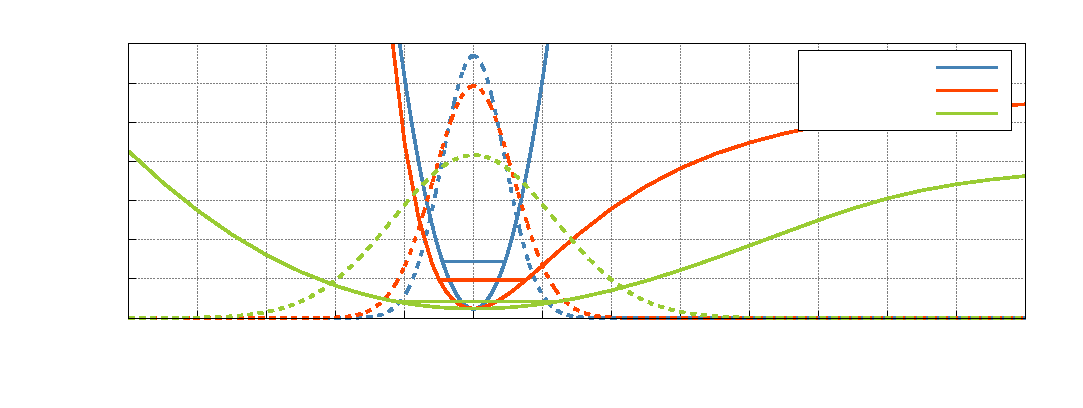
\includegraphics{4S-potentials}}%
    \gplfronttext
  \end{picture}%
\endgroup

    \vspace{-0.5\baselineskip}
    \caption{Diabatic, adiabatic and quantum potentials with associated wave functions and zero point energies in the harmonic approximation. The quantum potential is deduced from a harmonic fit of the wave function obtained from DFT with K treated quantum mechanically; the diabatic and adiabatic wave functions are obtained from a harmonic fit of the corresponding potentials}
    \label{fig:4S-potentials}
\end{figure}